%survey.tex
    %\brettcomm{BRING IN SOME MATERIAL FROM LIPTON, GUNNING, WELLER, AND DOSHI-VELEZ}
    %The definition given in Section~\ref{sec:assurances} gives a good definition and classification of assurances, but doesn't give very many practical insights into how assurances might be designed. 
    Whereas others have noted the \textit{existence} of assurances, we now directly consider the question: what, exactly, \textit{are} assurances, and how can they be \textit{practically designed} into AIAs? 
    This section surveys the related literature to understand what algorithmic approaches can be used to design AIA assurances. \nisarcomm{for me todo: make sure this lines up with end of previous Assurances section in background}
    
    \nisarcomm{not sure about this parag - necessary??}
    Figure~\ref{fig:refined_assurances} combines material from Section~\ref{sec:definitions} in order to make a more detailed version of Figure~\ref{fig:SimpleTrust_one_way}. In this section we perform a survey of the methods of calculation that have been used in literature. We have distilled the common concepts down to the following different approaches that will be discussed further.

    \begin{figure}[b]%[htbp]
        \centering
        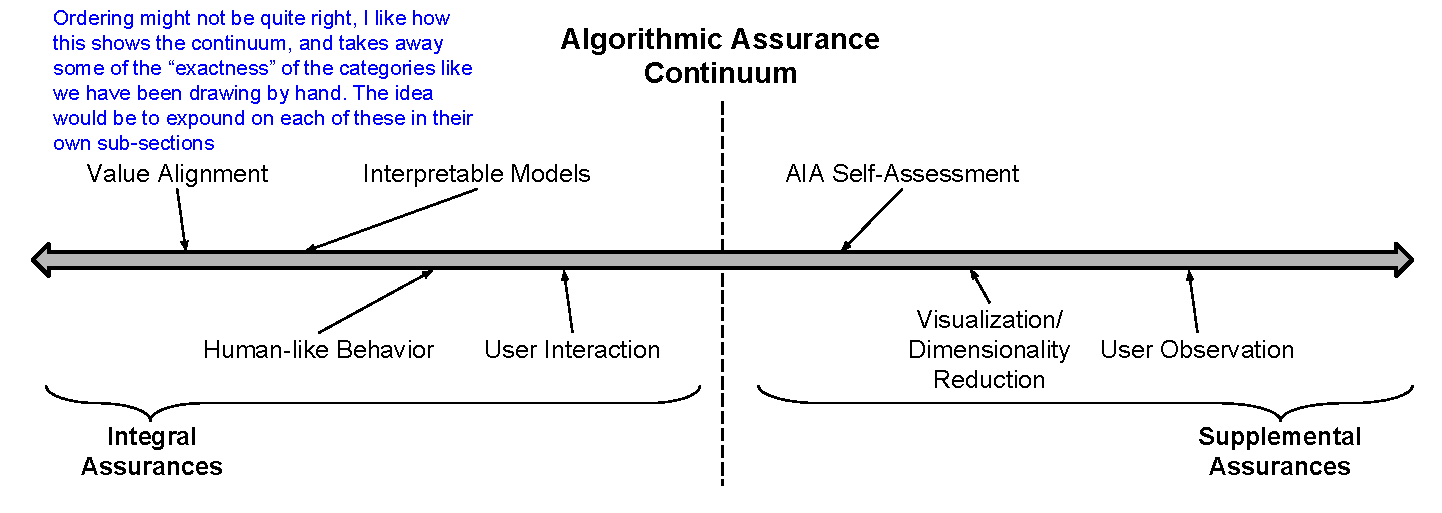
\includegraphics[width=0.85\textwidth]{Figures/Algorithmic_approach.pdf}
        \caption{Figure depicting the continuum of Algorithmic assurances. To the left are `Integral Assurances' that are integral to the key functions of the AIA. On the left are `Supplemental Assurances' that are supplemental to the key functions of the AIA. \nisarcomm{to be updated} }
        \label{fig:assurance_continuum}
    \end{figure}
\nisarcomm{note: generally should keep figures only on top and bottom of pages, as matter of style}

\subsubsection*{Survey Methodology} \label{sec:methodology}
    While theoretically a two-way trust model could be considered (i.e. in which the AIA also has trust in the user), attention is restricted here to a one-way trust relationship that considers only how user trust (and TRBs) evolves in response to assurances from the AIA. 

    It should be noted that it is practically impossible to perform a fully comprehensive survey of all AIA assurances, due to the broad spectrum of possible assurances, and AIAs in general. As an example, one could rightly argue that control engineers treat metrics like gain and phase margins as assurances for automatic feedback control systems, in much the same way that machine learning practitioners treat training and test accuracy as assurances for learning algorithms---and hence concepts related to robustness, stability, etc. for feedback control systems ought also be included in this survey. Similar arguments for assurances developed for fields like econometrics, software testing, aeronautical engineering and many others. While assurances can, in theory, be applied in both the most simple `automatic' systems (like a thermostat), this survey will focus on assurances in more advanced AIAs that make decisions under uncertainty. However, the admittedly narrow scope of this survey does not impede the development of fundamental insights and principles in designing assurances.

    Initially, in order to find applicable research, papers that formally addressed trust, and tried to create models of it, were investigated. This was done with the aim of trying to understand how trust might be influenced. Secondly, literature regarding trust between humans and some form of machine entity was reviewed; this lead to research in fields like e-commerce, automation, and human-robot interaction. Third, research on `interpretable', `comprehensible', `transparent', `explainable', and other similar types of learning and modeling methods were examined. Finally, with that literature as a background, research disciplines investigating computational methods that can be useful as assurances, but in which trust itself is not the main focus, were considered. This information was then used to construct an informed definition and classification of assurances based on methods that are currently in use, or being investigated.
    
    We now proceed to discuss each of the categories from Figure~\ref{fig:assurance_continuum}, starting from the most integral to the AIAs core functionality and proceeding to the least integral.

\subsection{Value Alignment} \label{sec:value_alignment}
Here we define `value alignment' as the design of AIAs that such that they are aligned with human values. Value alignment is more commonly known as `AI Alignment' in AI research (see \cite{Yudkowsky2001-hb,Bensinger2014-ul}), but we refer to it as value alignment as it is more clear in the context of assurances. \citet{Gordon_Worley2018-xy} states: ``\ldots the problem of AI alignment is to produce AI that is aligned with human values\ldots''. An AIA with aligned values will be considered by users to be more predictable (and thus more competent), because the AIA will be more likely to act in expected, `natural', ways.

\subsubsection{Common Approaches:}
Generally value alignment is concerned with the following topics (see \cite{Gordon_Worley2018-xy,Amodei2016-xi}): Negative side effects, reward hacking/gaming, scalable oversight and absent supervisors, safe exploration, robustness to distributional shifts, safe interruptibility, self modification, robustness to adversaries, ontology, idealized decision theory and logical uncertainty, vingean reflection, corrigibility, and value learning~\footnote{Readers interested in detailed descriptions of these categories should see \cite{Gordon_Worley2018-xy,Amodei2016-xi}}.

Among the more directly applicable topics in the scope of this paper are: reward hacking/gaming (taking advantage of imperfections in specification), safe exploration (how to learn in a safe manner), robustness to distributional shift (a difference between training data and test data), and design/learning of appropriate objective functions \cite{Hadfield-Menell2016-ws,Da_Veiga2012-gh,Garcia2015-rs}.

Some of these topics are not yet well formalized, however progress is being made, here we review some of the more practical approaches.

\paragraph{Reward Hacking/Gaming:}
Reward hacking is what happens when the rewards for an AIA are based on flawed specifications, or objective functions (such as objective functions with loop-holes). A popular example from \citet{Bostrom2014-fz} (roughly summarized here) is a robot that has an objective of making paper clips, it then decides to take over the world in order to maximize its resources and ability to make more paper clips; this highlights the point that sometimes `simple' objective functions can result in unintended/unsafe behaviors.

Even humans tend to reward hack/game, so the problem is far from solved. However, researchers have made use of practical approaches to attempt to align the values of AIAs with those of human users. One approach is to involve a human in the actual learning process. By doing so the human is able to encode a, possibly complex, objective function into the AIA. In theory, this provides an indirect way for users to build trust in the learning process by better understanding the `machine's perspective' (i.e. getting a sense for what it knows and doesn't know) and enabling mutual `calibration' of human-machine reasoning (rather than allowing users to simply attribute human understanding and learning processes onto the machine).

For instance, \citet{Freitas2006-qo} compared two approaches to discovering `interesting' knowledge from large data sets, based on the idea that human users require assistance from complex systems in order to find useful patterns and other interesting insights. He mentions `user-driven' methods that involve a user suggesting interesting templates or providing general impressions in the form of IF-THEN rules. These are then compared to different `data-driven' methods, using other research to suggest that data-driven approaches are not very effective in practice.

Having said that, user-driven approaches may not fare any better when compared over many users, as each user will likely have different preferences. Other scaled up user-driven approaches, e.g. based on crowd-sourcing \citet{Chang2017-kl}, can also achieve better accuracy for labeling tasks while also exploring new or ambiguous classes that can be ignored with traditional approaches (especially if training data sets are biased or very limited). \citet{Chang2017-kl} also consider a similar, scaled up, `user-driven' approach called `Revolt' that crowd-sources the labeling of images. It is able to attain high accuracy labeling, while also exploring new or ambiguous classes that can be ignored with traditional approaches.

\paragraph{Safety:}
While a fairly high-level treatment, \citet{Amodei2016-xi} are concerned with `AI safety', which is in essence: how to make sure that there is no ``unintended and harmful behavior that [emerges] from machine learning systems''.

Another related field is safe reinforcement learning (safe RL), which considers reinforcement learning is environments where failure is extremely costly, such as when using an expensive aerospace vehicle. Safe RL is a particularly important area that requires assurances, as the systems are designed specifically to evolve without supervision. \citet{Garcia2015-rs} perform a survey about safe RL highlight two main methods: 1) modification of the optimality criterion with a safety factor, and 2) modification of the exploration process through the incorporation of external knowledge. They present a useful hierarchy of approaches and implementations.

As one example, \citet{Lipton2016-dq} design an `intrinsic fear' RL approach that uses a deep Q-network (DQN) and a `supervised danger model'. The danger model stores the likelihood of entering a catastrophe state within a `short number of steps'. This model can be learned by detecting catastrophes through experience and can be improved over time. \citet{Curran2016-ij}, in a more specific application, asks how a robot can learn when a task is too risky, and then avoid those situations, or ask for help. To do this, they use a hierarchical POMDP planner that explicitly represents failures as additional state-action pairs.

Finally, moving on from ML-oriented approaches, one can also consider approaches rooted in Validation and Verification (V\&V). V\&V typically refers to the use of formal methods to guarantee the performance of a system within some set of specifications. However, not all practitioners are aware that V\&V provides ways to assure users. A prime example is given by \citet{Raman2013-mz}, who developed a way by which a user can provide natural language specifications to a robot and a `correct-by-construction' controller will be built if the specification is valid. Otherwise, the robot will provide an explanation about which specification(s) will cause failure. This approach is studied with the goal of implementing the system on a robot assistant in a hospital. Their method involves parsing natural language input (``Go to the kitchen''), and converting that into a linear temporal logic (LTL) task specification. This is then used to synthesize a robot controller if possible; otherwise, the `unrealizable' specifications are communicated back to the user. This approach is promising in that it presents a way to communicate that a specification cannot be met. But, it does not formally account for effects on user trust or TRBs in formulating explanations. The expression of assurances is also asymmetrically limited to cases where the robot cannot meet the specifications. 

In the context of a practical self-driving car application, \citet{Ghosh2016-dl} presents a framework called Trusted Machine Learning (TML) for making ML models fit pre-determined `trustworthiness' constraints. Unlike most other kinds of assurances considered so far, these constraints are handed down by a certification authority as requirements to the ML system designer, and are not meant to be exposed to/determined by users. However, in principle, such hard assurances could be exposed to users in certain contexts. The key idea is to utilize tools from formal methods to provide theoretical proof of the functionality of the system. Note that, in the formal methods literature, such proofs and their supporting evidence are what are referred to as `assurances'; we earlier denoted these as `hard assurances', in contrast to the other kinds of `soft assurances' considered here. 

\paragraph{Learning Under Nonstationarity:}
Learning under nonstationarity refers to the real challenge of training a model based on data from one distribution while taking into account that the test distribution will likely move (i.e. be nonstationary) or `shift' through time. \citet{Quinonero-Candela2009-fj} address many different aspects of this problem.

\citet{Sugiyama2013-ci} suggest approaches for addressing 1) `covariate shift' (training and test input data follow different distributions), and 2) `class-balance change' (where the class-prior probabilities are different in training and test phases, but where there is no covariate shift). A key approach to addressing both problems is to use `importance sampling' which involves weighting the training loss according to the ratio between $p^\prime(x)$ and $p(x)$; this ration is referred to as the `importance'. \citet{Charikar2017-kr} address the problem of learning from `untrusted' data; this data could be untrusted due to adversarial attack or nonstationarity.

\brettcomm{add some references about robust estimation and control?}

\subsubsection{Grounding Example:}
In the case of the `VIP Escort' problem (described in Section~\ref{sec:mot_example}), value alignment might be used as an assurance in the following way:

We make the following assumptions

\begin{itemize}
    \item The UGV has just begun an attempt to escape the road-network
    \item The UGV uses safe RL to learn its escape policy
    \item The operator is able to observe the UGV during its entire escape attempt
\end{itemize}

The operator has used several different UGVs for similar tasks. This newer model uses `safe RL' to learn its policy. When observing the UGV's attempt at escape the operator notices a difference in how the UGV operates. Whereas the older UGV models would sometimes do risky things, this UGV seems to avoid dangerous situations much better. 

\paragraph{\textbf{Discussion of Example:}} In this case, safe RL enabled the UGV to treat situations that an operator might classify as `dangerous' with more care. With this integral capability the UGV assures the operator that it is more competent.

\subsection{Interpretable Models} \label{sec:interp_models}
we want these here: \citet{Chipman2005-om, Morrison2016-fz, Van_Belle2012-dt, Park2016-ld, Jovanovic2016-gw, Choi2016-by, Huysmans2011-th, Caruana2015-za, Faghmous2014-og, Ruping2006-xj, Lipton2016-ug}

\subsection{Human-Like Behavior} \label{sec:human_behavior}
Since humans are accustomed to forming and evaluating trusting relationships with each other, imitation of human-human communication and interactive behaviors provides yet another avenue for developing AIA assurance strategies. 
Support for this idea is given by \citet{Tripp2011-rx}, who compared human trust in other humans against human trust in intelligent interactive technology. 
They found that, as the technology becomes more `human-like', self-reported levels of trust in technology become more similar to levels of trust in other humans.

\citet{De_Visser2018-kd} also specifically discusses different methods by which AIAs can be more human-like in order to `repair trust' with users (here, trust repair is roughly analogous to assurances, but focuses on re-building trust after it is lost). Among several other possibilities, they suggest that an AIA might repair trust by anthropomorphizing (responding using a human communication channel), or by explaining its actions in the same way a person would. 
Such human-like behavior opens the door for AIAs to exhibit `non-rationally motivated' behaviors (i.e. suboptimal, as opposed to irrational actions), if these conform to social norms or other psychological cues that provide useful assurances about predictability (e.g. a robot arm that executes legible motions), competency (e.g. a robot which slowly backs away from unfamiliar or potentially dangerous objects), or situation normality (e.g. a robot car that apparently rubbernecks near an unfamiliar scene on the road). 

\subsubsection{Common Approaches}
Generally, we do not have algorithms that describe how humans interact with each other (yet), and must settle for heuristics or best attempts to create human-like behavior via algorithms. From a high level, researchers have addressed these: nonverbal communication, and mannerisms.

\paragraph{Nonverbal Communication:} 
Nonverbal communication can take many different forms. One popular approach is to use motion or gestures. \citet{Szafir2014-ok} investigated how to enable `Assisted Free Flyer' robots (quad-copters that are made to interact with humans in close spaces) to communicate by using gestures. In doing so they use `motion primitives' (a basic vocabulary of movements) that were inspired by basic `character animation' principles \cite{Van_Breemen2004-rz}. 
In their evaluations of these primitives with human participants in the presence of free flyers, they found that human users significantly found the free flyers to be more natural, and felt safer around them. Later \citet{Szafir2015-iy} also experimentally showed the effectiveness of using illuminated `turn signals' and pairs of human-like `eyes' that shifted with free flyer heading (much as human eyes do when people walk in a crowd) to help users more easily interpret the vehicle's intended movements and actions. These works provide strong support for `commonsense communication' assurances aimed at predictability in physical user-AIA interactions (even if indicators like `moving eyes' do not actually see anything). 
Likewise, \citet{Dragan2013-wd} investigate `legible motion planning', i.e. planned robotic physical movements and gestures that, by themselves, convey intended actions and goals. For example, a table-setting robot may grasp a plate on both sides from the top using two end effectors if it intends to shift the position of the plate along the table surface, whereas it may grasp the same plate with only one hand from the side if it intends to pull away and remove the plate from the table. 
Legible motion is used by humans working in close proximity, and so can also be useful and important for situations in which a physically embodied AIA and person are collaboratively working in close proximity to each other. Similarly, in more recent work \citet{Kwon2018-xt} investigates calculating trajectories that convey `incapability', which is \emph{what} the AIA is trying to do, and \emph{why} it is unable to do so. 
See also \cite{Admoni2016-db} for related work. 

\paragraph{Mannerisms:}
Humans are naturally inclined to leverage social interaction cues and adherence to/violation of social norms as evidence for assessing the trustworthiness of other humans in everyday interactions. 
AIAs can leverage these inclinations to provide simultaneous assurances of their competence, predictability, and situation normality. 
Consider, for instance, a recent `mini-Turing Test' example from the popular media: at Google/IO 2018, Google Duplex \cite{Google2018-eb} was introduced through a demo where it placed a phone call to make a reservation. 
An oft-remarked feature of this demo is the great difficultly (if not near impossibility) of detecting whether or not the Duplex voice is human -- down to the words spoken, tone of voice, and speech mannerisms (which included `um\ldots', pauses, and shortened sentences). 
The human on the other end of the call was none the wiser, and trusted that they were in fact speaking to a regular human customer -- when in fact they were speaking in a completely natural manner to the product of a recurrent neural network (RNN) trained on anonymized phone conversation data. 

More formally, \citet{Salem2015-md} investigated the effects of autonomous task errors, task types, and `system personality' on cooperation and trust for humans who observed a domestic robot performing house tasks, such that the robot implicitly showed competence by its mannerisms and successes/failures during tasks. In this case, the mannerisms and competency of the robot were completely under control and hard-coded into the system. Regardless, when participants were asked to cooperate with the robot on certain other tasks, the strange/unexpected operation of the robot was found to influence the self-reported trust levels of the participants.

\citet{Wu2016-ei} investigated how a person's decisions in a coin entrustment game are affected by their belief in whether they are competing against an AIA or another human player (which, unbeknownst to participants, was in fact an AI with some programmed human-like idiosyncrasies, e.g. variable wait times between turns). Trust in this context was measured directly by the number of coins a participant was willing to lose by putting them at risk to the other player. The experiment found that the participants trusted the AI opponent more than they trusted the `human' opponent; the authors suggest that this may be due to the perception that the AI opponent did not have feelings and operated in a more predictable and consistent `machine-like' way. Given that the `human' was an AI as well, this experiment illustrates that `machine-like' behavioral consistency can lead to implicit positive effects the trust of the participant in certain contexts.

\subsubsection{Grounding Example:}
In the case of the `VIP Escort' problem (described in Section~\ref{sec:mot_example}), human-like behavior might be used as an assurance in the following way, starting with the assumptions that:

\begin{itemize}
    \item The UGV is about to begin an attempt at escaping the road-network
    \item The operator can observe all the actions of the UGV via video feeds at intersections
    \item The UGV has been designed with the ability to use gestures in order to indicate its `incapability' as in \cite{Kwon2018-xt}
\end{itemize}

As the UGV begins the escort problem, the human supervisor is monitoring progress. As the UGV reaches a certain intersection of the road network the supervisor expects the UGV to take a path $A$, but it does not. However, before choosing to take path $B$, the UGV made a movement that, to the operator, indicated that it considered attempting to traverse $A$. Due to the attempt the supervisor was able to surmise that the UGV wanted to take that path but couldn't due to some limitation.

\paragraph{\textbf{Discussion of Example:}} In this case the UGV is able to maintain appropriate trust of the supervisor because the supervisor was able to interpret the `gesture' that UGV was using. This highlights the assuring effects that human-like communication/behaviors can have on users.

\subsection{User Interaction} \label{sec:user_interaction}
To date one of the more common approaches to engender trust in users has been to put the users `in-the-loop'. This has been, and still is, modus operandi in the automation industry and others. While some think that more advanced AIAs will `soon' be able to operate with little human involvement, those who have more practical experience with them are more reserved.

In this section we review some methods by which engineers have made AIA assurances by making the performance of the system highly dependent on the user's participation. This includes work from disciplines such as human-robot collaboration, cooperative control, cooperative sensing, and others. This is analogous to a supervisor working `in the trenches' with those they supervise; in doing so they are able to provide feedback in real-time and better appreciate the decisions and outcomes that take place.

\subsubsection{Common Approaches:}
\nisarcomm{what are the main ideas to cover beyond the individual papers? first talk about what *could* be done in terms of human roles (humans as planners/controllers, sensors/perception augments, tutors/trainers, etc.) -- then discuss how each approach contributes to acting as an assurance for an AIA, using refs as specific examples -- otherwise a laundry list of papers doesn't really help organize or convey any part of your argument here }\brettcomm{In what ways can users interact? make a list. Humans as sensors, humans as controllers,\ldots}

\paragraph{stuff:}
\citet{Sweet2016-dw} investigate how to enable using humans as `soft' sensors, and then fuse their input into the `hard' robot sensors to improve and augment the robot's Bayesian state estimation capabilities. They apply their approach in a scenario they call `cops and robots' where a single `cop' robot tries to locate `robber' robots. In this case the human acts as a deputy that remotely interacts with the system. The human can see security camera footage of the building in which the cop is searching and can offer natural language feedback to the cop robot when appropriate. If the human offers information it can be fused into the cop robot's estimation model, but in the meantime the cop robot operates autonomously without assistance.

Similarly \citet{Tse2015-tz} consider a framework for robots and humans to share and fuse information in a cooperative context. \nisarcomm{so...? there's a lot more to be said here...}

\citet{Tellex2014-uc} consider an autonomous assembly robot that can detect when it has failures (expected conditions that don't match expectations). When this occurs the robot requests help from the human user to resolve the problem. In this way the human and robot are dependent on each other to accomplish a task.\ldots I'm not sure if this one belongs either.

\citet{Kaupp2008-yr,Kaupp2005-pk} identify the appropriate level of automation for a system while taking into account the amount of interaction required by a human operator. In this case the robot has sensors of its own, but can also ask for user input when the value of information (VOI) is high enough; they define the threshold VOI by human trials before deployment of the system in order to optimize the involvement of the human user.

\citet{Freedy2007-sg} studied how mixed-initiative human-AIA teams might have their performance measured, and examined the extent to which such teams can only be successful if ``humans know how to appropriately trust and hence appropriately rely on the automation''. 
They explore this idea by using a tactical reconnaissance scenario where human participants supervised an unmanned ground vehicle (UGV)  platoon with three levels of autonomous targeting/firing capability (low, medium, high); these levels were dependent on the experimental conditions. The operator needed to monitor the UGV in case it couldn't perform as desired.
Operators were trained to recognize signs of task failure, and to only intervene if they thought the mission completion time would suffer. Trust was formally acknowledged in this survey and was quantified by using the Relative Expected Loss (REL) measure, which is the mean number of trials to expected loss of robot control over $n$ experimental trial runs. 

\subsubsection{Grounding Example:}
In the case of the `VIP Escort' problem (described in Section~\ref{sec:mot_example}), operator interaction might be used as an assurance in the following way:

We make the following assumptions

\begin{itemize}
    \item The UGV has just begun an attempt to escape the road-network
    \item An interface system exists by which the operator can provide information to the UGV
\end{itemize}

The UGV is capable of operating autonomously, but also has the ability to ask for assistance or information when necessary. In this way the functionality of the UGV ca be greatly improved via interaction with the user. As the user interfaces with the UGV and is able to provide feedback and information about the best known location of the pursuer based on information unavailable to the UGV they have more trust in the competence, predictability, and situational normality of the UGV.

\paragraph{\textbf{Discussion of Example:}} In this scenario the user is more immersed in the functioning of the UGV. Not only are they able to respond to queries from the UGV, but they can also provide direct observations as well. In this way the user feels more immersed in the functioning of the UGV and is more cognizant of appropriate TRBs.

%%(i) assurance argument: what specifically is the assurance signal/rationale? -- whereas user interaction techniques of previous section generally tend to provide integral assurances (i.e. designed as part of core functionality of AIA capabilities) that introspectively compensate for shortcomings in AIA capabilities, similar introspective assurances can also be generated to determine and inform users of competency limits/boundaries of AIA capabilities *without requiring* user interaction or intervention -- and thus can be considered as supplementary to or separate from core AIA functionality. That is:  assurances can be provided to introspectively determine and explain/interpret limits of what AIA can do or knows, etc. for the sake of the user, without requiring modification of underlying AIA design.  In this sense, self-assessments can provide users with insights on one or both of the following related concerns: what can the AIA actually do and what does it know? and, what is required of/by the AIA to actually do the assigned task?  The first concerns identifying set of tasks in `reach set' of AIA; the second concerns figuring out what would be needed to do current task [need to refine this...trying to distinguish between questions that lead to insights about competency and situation normality via complexity reduction, vs. insights that inform predictability via uncertainty]... but basic analogy [can be mapped to UGV] is subordinate/delegate telling supervisor what it is/is not capable of, vs telling supervisor what it would need to be able to carry out specific task at hand or what the possible outcomes would be for that specific task (so, self-assessment can have contrasting focus on AIA itself on general capabilities vs. on the task at hand in relation to how AIA would perform on it specifically)...
%%(ii) what is mechanism for generating appropriate TRBs? -- Key targets are competency and situational normality dimensions in terms of explaining AIA functionality, whereas predictability is key target for task oriented assurances. Assurances from self-assessment paradigms are typified by frameworks like `machine self-confidence'[] and explainable Bayesian inference[] -- these operate on the results of `black box' AIA component outcomes in a post hoc manner, unlike interpretable models discussed earlier (which force AIA components to be inherently `understandable' to users). Viewed differently: whereas interpretable models are more `bottom up', self-assessment is more of a `top down'/drill down process: latter is less constrained in choice of models/techniques for AIA capabilities, but also must rely on ability to suitably decompose these same AIA functions across different task contexts and 
%%(iii) how can designers build/exploit for AIA assurances, i.e. what techniques available for getting assurances from self-assessment?: 
%%(a) complexity reduction...  
%%(b) uncertainty...


\subsection{AIA Self-Assessment} \label{sec:aia_self_assessment}

\subsubsection{Common Approaches:}
\nisarcomm{Need to say a bit more about what the motivation/general idea here is, to continue flow from other previous sections...}
The literature in this category can be split into two high-level categories. The first concern is for an AIA to be able to account for its uncertanties (i.e. uncertainty in its models of its world, sensors, and capabilities). The second is to attempt to reduce its complex, `uninterpretable', capabilities into more interpretable ones.

Here the AIA makes an active attempt at processing data and making information available to the user. This is done in a post-hoc manner, or in a way such that the quantification of uncertainty is more supplemental, rather than integral, to the main functions of the AIA.

\paragraph{Quantify Uncertainty} \label{sec:QU}

Although active learning does not explicitly consider safety, the underlying approaches can be useful because active learners need to be able to search the problem space to reduce uncertainty; this requires an internal representation of uncertainty. The applications surveyed here are all mainly related to image classification and robotics. In the context of image classification, \citet{Paul2011-vr} introduced `perplexity' as a metric that represents uncertainty in predicting a single class and is used to select the `most perplexing' images for further learning. There have also been several attempts to use Gaussian processes (GPs) to actively learn and assign probabilistic classifications \cite{MacKay1992-sp,Triebel2016-kj,Triebel2013-ow,Triebel2013-ku,Grimmett2013-gj,Grimmett2016-yc,Berczi2015-rd,Dequaire2016-kh}. As with perplexity-based classifiers, the key insight is that if a classifier possesses a measure of uncertainty, then that uncertainty can be used for efficient instance searching, comparison, and learning, as well as reporting a measure of confidence to users. The key property of GPs to this end is their ability to produce output confidence/uncertainty estimates that grow more uncertain away from the training data. This information can be readily assessed and conveyed to users, even in high-dimensional problems. This property has also found much use in other AIA active learning problems, e.g. Bayesian optimization \cite{Snoek2012-tt, Brochu2010-tj,Israelsen2017-zb}. 

\citet{Choi2017-th} investigates how mixture density networks (MDNs)---neural networks that learn parameters of a Gaussian mixture distributions---can be used to help a controller switch modes based on the MDN's prediction of 

Bayesian neural networks (BNNs) are a method by which we can have insight into the uncertainty of a neural network model. Using BNNs \citet{Kendall2017-ry}, in the context of computer vision, also use deep BNNs to help visualize epistemic (input) and aleatoric (model) uncertainty for each pixel of an image. 

Similarly \citet{Kahn2017-vy} use deep BNNs to learn about the probability (with uncertainty) of an autonomous vehicle colliding in an environment given its current state, observations, and sequence of controls. Using this model they formulate a `velocity-dependent collision cost' that is used for model-based reinforcement learning. With this approach the vehicle naturally proceeds slowly when there is an elevated risk of collision. \brettcom{not sure if this goes here, or in the `value alignment' section\ldots it goes here if i downplay the built-in nature of the behavior, and instead focus on the ability to quantify uncertainty}

An AIA that can predict its performance on different tasks can provide assurances about competence, predictability, and the situational normality of a given task. Several authors have worked to improve this ability in visual classification \cite{Zhang2014-he,Gurau2016-hs,Churchill2015-ei,Kaipa2015-hy}. 
For example, to ensure that visual classifiers don't fail silently in novel scenarios, 
\citet{Zhang2014-he} learned models of errors on training images to predict errors on test images. 
\citet{Kaipa2015-hy} consider 3D visual classification of assembly line parts for robotic pick and place tasks, and develop statistical goodness-of-fit tests to estimate the likelihood that robots can use their sensors to find parts matching desired ones. %To accomplish this they apply the `Iterative Closest Point' (ICP) method, to match a point cloud measurement of the part with a ground-truth 3D model of the part. 
These approaches allow the AIA to assess capability and present appropriate assurances to users, though without any formal notions of trust. 

Models and logic are not trustworthy by themselves; they may be flawed to begin with, or become invalid when certain assumptions or specifications are violated. Thus, there is great interest in providing assurances that the models and assumptions underlying different AIA processes are in fact sound. \citet{Laskey1991-mf} -- with the intention of communicating model validity to users of `probability-based decision aids' -- notes that it is infeasible to perform a decision-theoretic calculation to determine if model revision is necessary. 
She presents a class of theoretically justified model revision indicators which are based on the idea of constructing a computationally simple alternate model and then initiating model revision if the likelihood ratio of alternate model becomes too large (see also \citet{Zagorecki2015-qy,Habbema1976-xd} --these ideas also provide a potential basis for the `model validity' machine self-confidence factors from Quadrant II).
\citet{Ghosh2016-dl}  present `model repair' and `data repair' strategies that can be used when the current model doesn't match the observed data, at which point the model and data can be repaired, and control actions can be replanned in order to conform with the formal method specifications. One challenge is how the `trustable' constraints should be identified, as this places a strong burden on the certifying authorities and system designer to foresee all possible failures.


\paragraph{Reduce Complexity} \label{sec:reduce_complexity}
Representations within an AIA are often complex. Sometimes using inherently less complex, `interpretable models' (as discussed in \ref{sec:interp_models}), is the most straight forward way to address this challenge. However, in some cases it is desirable to maintain complex, less interpretable representations (e.g. for performance reasons) and then reduce the inherent complexities (possibly post-hoc) to aid human users.

One typical approach is to generate explanations, but how should explanations be provided? There are also considerations regarding whether explanations should occur by two-way interaction between system and user, by natural language interaction, or by probabilities. Some of the answers to these questions lie more in the realm of cognitive science. Still, natural language and other communication modalities could be used~\cite{Hayes2017-nt}. Specifically, \citet{Olah2018-rp} investigate how predictions of NNs can be explained through visualizing how different parts of the network respond to certain images. They propose combining several different approaches to get a holistic view of the NN behavior. Specifically, they use feature visualization (what a neuron is looking for), and attribution (how it affects the output).

There are several classes of explanations. \citet{Abdollahi2018-uw} propose three in the context of collaborative filtering: `neighbor style' (explanation based on examples from similar situations), `influence style' (present the most influential items that led to a certain model output), and `keyword style' (identify common features between user keywords, and content). \citet{Otte2013-oo} and \citet{Ribeiro2016-uc} implement analagous ideas in the realm of safe ML and interpreting classifiers respectively. 
\citet{Huang2017-lk} use `algorithmic teaching' (see~\cite{Balbach2009-jw}) as inspiration for helping human users learn a robot's true objectives. Algorithmic teaching involves having a model of a students learning algorithm, and then presenting training examples to allow the student to learn a target model. In this case the `student' is the human user, and the `teacher' is the robot that is trying to teach the human its own objective function by presenting a set of (optimal) training examples. Here we would consider the robot's training examples as assurances.

Another consideration is whether an explanation is meant to be descriptive or aimed at ensuring comprehension, as well as whether explanations need to be on a macro or micro scale relative for parts of the Bayesian network (similar to globally/locally interpretable learned models \cite{Ruping2006-xj}). 
\citet{Lacave2002-cu} address the AIA reduction of complexity from the perspective of explaining probabilistic inference in Bayesian networks---specifically, \emph{how} and \emph{why} a Bayesian network reaches a conclusion given some imputed evidence. 
They present three properties of explanation: 1) content (what to explain), 2) communication (how to explain), and 3) adaptation (how to adapt based on who the user is). Several key points for designing assurances arise from considering the differences between explaining evidence (i.e. data), the model (i.e. the Bayesian network itself), or the reasoning (i.e. the inference process).

\citet{Aitken2016-cv} propose a metric called `machine self-confidence' for providing users with better insight into autonomous decision making under uncertainty. This insight comes from breaking down the complex influences of uncertainty on the decision making process and presenting them to the user in a simple way. Self-confidence is defined as the machine's own perception of its ability to carry out tasks in light of uncertainties in its knowledge of the world, its own self/states, and its reasoning process and execution abilities. In this sense, self-confidence is an AIA's metacognitive assessment of its own behavior and `competency boundaries'. A computational measure for POMDP-based autonomous planning is defined from five component assurances (which are fairly general and applicable to most other kinds of planners): 1) Model Validity, 2) Expected Outcome Assessment, 3) Solver Quality, 4) Interpretation of User Commands, and 5) Past Performance. 
The key idea behind this set of measures is to assess where and when approximations required for planning under uncertainty are expected to break down. Model validity attempts to quantify the validity of a model within the current situation. The expected outcome assessment uses the distribution over rewards to indicate how beneficial or detrimental the outcome is likely to be. Solver quality quantifies how a specific POMDP solver is likely to perform in the given problem setting (i.e. how close to optimal the solution policy and approximate solution policy can get). The interpretation of commands component is meant to quantify how well the objective has been interpreted (i.e. how sure is the AIA that it correctly interpreted mission specifications into relevant tasks and suitable goals). Finally, past performance is meant to add in empirical experience from past missions, in order to make up for theoretical oversights and account for learning-based processes.

\citet{Aitken2016-cv} proposes that self-confidence values could, for instance, be reported as a single value between $-1$ (complete lack of confidence in achieving mission objectives) and $1$ (complete confidence in achieving mission objectives); a self-confidence value of $0$ reflects total uncertainty. Each of the component assurances could be useful on its own, but the composite `sum' of the factors is meant to distill the information from the five different areas, so that a (possibly novice) user can quickly and easily evaluate the ability of the AIA to perform in a given situation. Currently, only two of the five metrics (Expected Outcome Assessment, and Solver Quality) have been developed quantitatively, but there is continuing work on the other metrics and they plan to perform human experiments to evaluate the usefulness of the self-confidence metrics for AIAs. Other approaches for computing and communicating AIA self-confidence have also been proposed for more specific applications \cite{Hutchins2015-if, Kaipa2015-hy, Zagorecki2015-qy, Kuter2015-qh}. 


\subsubsection{Grounding Example:}
In the case of the `VIP Escort' problem (described in Section~\ref{sec:mot_example}), self-assessment might be used as an assurance in the following way:

We make the following assumptions

\begin{itemize}
    \item The UGV is about to being an attempt to escape the road-network
    \item The UGV is using the `solver quality' metric mentioned by \citet{Aitken2016-fb}
    \item The operator has access to an interface where they can view the self-confidence metric calculated by the UGV
\end{itemize}

Before the UGV begins its attempt it is able to assess its `solver quality' given the specific, unseen road-network, based on similarities between the current network and ones that it has encountered before. The UGV reports that it has high confidence in its solver quality, and the operator is assured that they can trust the solver in this situation.

\paragraph{\textbf{Discussion of Example:}} In this case the UGV is able to assure the operator of the quality of the solver in the specific road-network. Generally, the UGV reduced what could be a very complex analysis into a simple format for the operator to interpret. This is in contrast to the operator viewing policies, models, algorithms, and complex probability distributions.

%%(i) assurance argument: what specifically is the assurance signal? 
%%(ii) what is mechanism for generating appropriate TRBs? 
%%(iii) how can designers build/exploit for AIA assurances, i.e. what techniques available for ...?: 
%%(a) ...  
%%(b) ...
%%(c) ...

\subsection{Information Visualization} \label{sec:vis_dr}
We define `information visualization' as the act of displaying information in such a way as to communicate to one of the trust dimensions of a human user. Specifically we consider the `competence', and `predictability' of the AIA and the `situational normality' of the task at hand.

\subsubsection{Common Approaches:}
\citet{Liu2017-xw} review several of the current methods that exist for visualizing ML models. They identified three main purposes for which visualizations are useful in this context: 1) understanding (why model behave how they do), 2) diagnosis (failures, or unexpected behavior), and 3) refinement (ability to improve performance). We focus on \emph{techniques} that assist in that process.

Two of the main tools in creating visualizations are and reducing the dimensionality, and treating uncertainty in creating the visualizations to assist users in understanding more easily.

\paragraph{Dimensionality Reduction:}
Dimensionality reduction (DR) is one of the key methods used in creating visualizations. \cite{Sacha2017-hf} identify seven different methods by which users interact with DR techniques. They use this to make the human-in-the-loop process model for interactive DR that is shown in Figure~\ref{fig:sacha_fig}.

\begin{figure}[htpb]
    \centering
    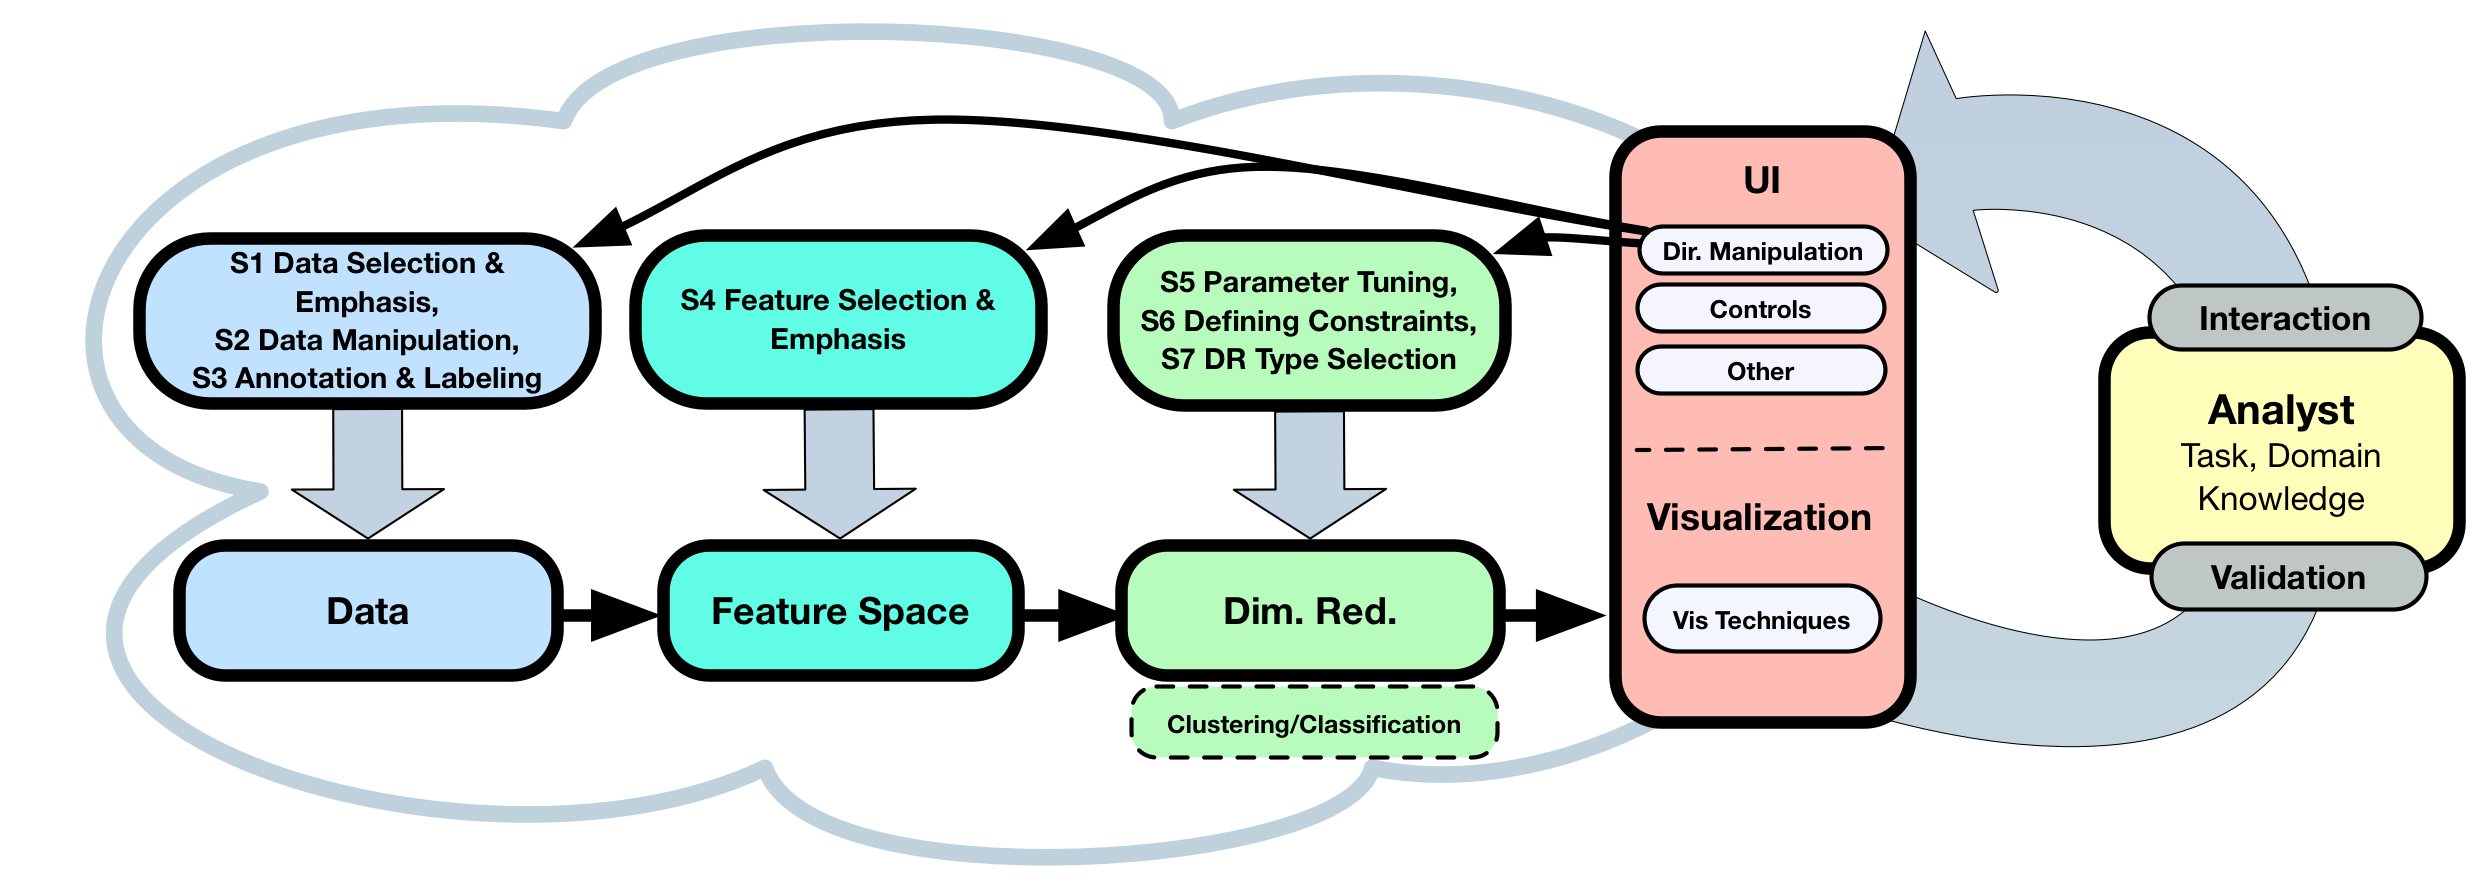
\includegraphics[width=0.9\linewidth]{Figures/dimred_framework.png}
    \caption{Human-in-the-loop process model proposed by \cite{Sacha2017-hf}. Included by permission.}
    \label{fig:sacha_fig}
\end{figure}

\citet{Venna2007-yj} discusses DR for ML and reviews many linear and non-linear projection methods. \citet{Vellido2012-nm} also discusses the importance of DR for making ML models interpretable. As one example, \citet{Chipman2005-om} applied this idea by constraining principle component analysis (PCA) in an attempt to make the resulting linear combinations of variables be more interpretable (more homogeneous, or more sparse).

At times a simple visualization is the most efficient way to communicate the results of decision making, planning. For example: \citet{Chadalavada2015-wx} enable a robot to project its path onto the ground so users can see.

\paragraph{Treatment of Uncertainty:}
In the previous section we have already visited the importance of an AIA being able to quantify its uncertainty. Visualization researchers are concerned with how to \emph{convey} that uncertainty to human users (and quantify uncertainty inherent in making visualizations). \cite{Sacha2016-tu} discuss how the propagation of uncertainty through visual analytics systems can affect the trust of human users (see also \cite{Correa2009-hi}).

One excellent example of this is the work by \citet{Wu2012-qi}, who create a tool to visualize the flow of uncertainty in the visualization process. In this way users can understand where uncertainty enters the visualization process.

\begin{figure}[htpb]
    \centering
    \includegraphics[width=0.6\linewidth]{example-image-golden}
    \caption{Example visualization of the flow of uncertainty in the creation of a visualization \cite{Wu2012-qi}. Included by permission.}
    \label{fig:hutchins_fig}
\end{figure}

The relationship between system uncertainty and the effects of uncertainty on the performance of the system can be very complex to understand. \citet{Hutchins2015-if} address this by using expert knowledge, and a `trust annunciator panel' (TAP) that has several `uncertainty level indicators' in order to display how uncertainties in sensors will effect the output quality, and the mission impact; and the same for the planning algorithm (see Figure~\ref{fig:hutchins_fig}).

\begin{figure}[htpb]
    \centering
    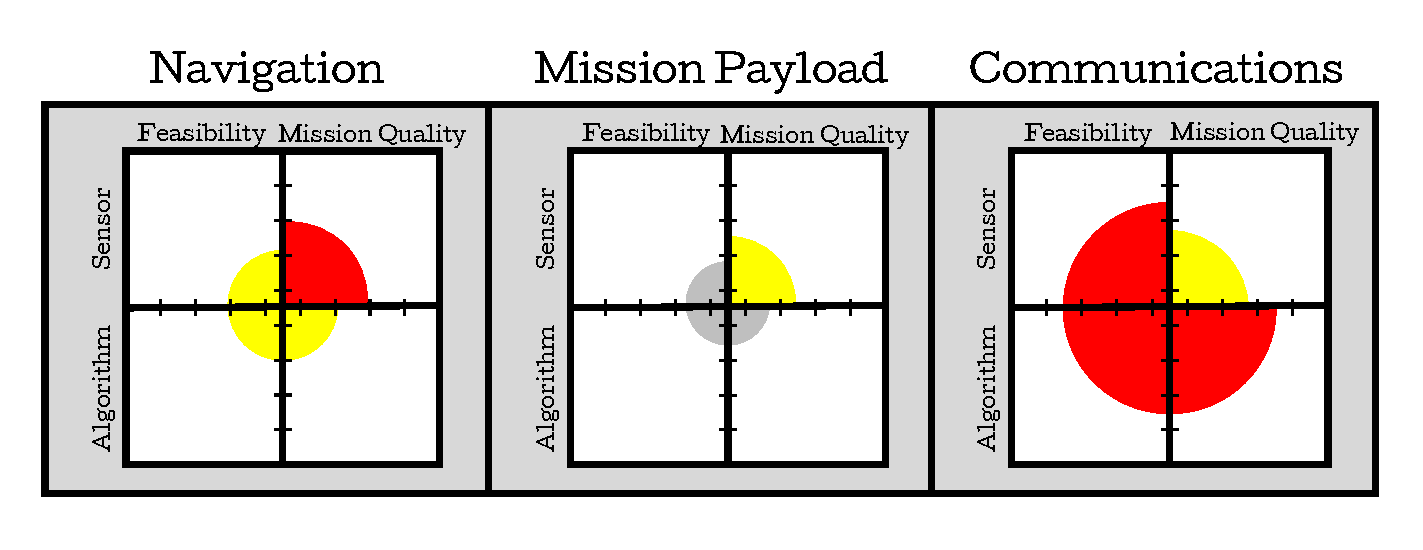
\includegraphics[width=0.9\linewidth]{Figures/Hutchins_fig.pdf}
    \caption{Proposed `trust annunciator panel' \cite{Hutchins2015-if}. Included by permission.}
    \label{fig:hutchins_fig}
\end{figure}

\subsubsection{Grounding Example:}
In the case of the `VIP Escort' problem (described in Section~\ref{sec:mot_example}), information visualization might be used as an assurance in the following way:

We make the following assumptions

\begin{itemize}
    \item The UGV has just begun an attempt to escape the road-network
    \item The user has access to an interface like that proposed in \cite{Hutchins2015-if}
\end{itemize}

During the attempt the user is able to see how the sensor uncertainty might possibly effect the outcome of the mission. In this case, the user is assured that the sensors will have little negative impact on the outcome of the mission given the current weather conditions.

\paragraph{\textbf{Discussion of Example:}} Here we see how a visualization is able to assist the user in correlating the effects between sensor uncertainty and mission outcome. This is not a simple relationship for operators (especially untrained) to learn on their own; even if they were able to learn the time required to do so can be very detrimental.

\subsection{User Assessment} \label{sec:user_assessment}
In this section we address assurances that are based solely on user assessment; in other words the AIA expends little or no computational effort to `digest data' to turn into assurance information for the user, and instead relies the user's own cognitive abilities to draw assurances from their observations. Such assurances are clearly not integral to the function of the AIA, as they might, for example, be realized by incorporating simple displays, print statements, or other `raw data' indicators into a basic user interface. 
This category is in contrast to Section~\ref{sec:vis_dr}, where the AIA is designed to process data to assist the user in understanding how to trust the AIA appropriately. This approach is enticing for many system designers given how easy it is to implement at any stage of AIA design (even as an after-thought). However the effectiveness of this approach rests on several, strong, assumptions:

\begin{itemize}
    \item The user is capable of forming a `good enough' mental model of the AIA on their own to inform appropriate TRBs;
    \item Different users have `similar enough' capabilities and experiences to draw appropriate inferences on their own;
    \item There are no other compelling sources of information that will confound the assurance;
    \item Common cognitive biases won't interfere with the long-term operation/supervision of the system (e.g. recency, framing or anchoring effects that skew user's perception of non-linear changes in performance variables like power/fuel consumption). 
\end{itemize}

The weight of each of these assumptions relies heavily on the task to be performed, and the characteristics of the typical users. For example, in situations with highly trained personnel (i.e. military, or manufacturing facility) all users will have similar level of capability; thus `user assessment' is a viable and effective solution. 
In other scenarios with more diverse users and operating environments these assumptions being to break down. 

\subsubsection{Common Approaches:}
As suggested in the section's name users can form assurances by any method of perception. The most commonly investigated approach is by simple, visual, `display of raw data', and `by inspection' performance-based assessment. %%Other forms of human perception are not well investigated in this context, but work in perception of businesses and products for marketing is probably very applicable.

\paragraph{Display of Raw Data:}
Assurances associated with displaying AIA performance variables sound banal (e.g. flow rate for an automated pump \cite{Muir1996-gt}), but actually involves a nuanced point: the displayed performance value actually serves to inform the user's own mental model of the trustworthiness of an AIA capability. That is, the user's trust in the AIA's capability does not change only in response to the instantaneous `goodness/badness' of the AIA's performance, but accounts for the past history of the AIA's performance as well as any observed discrepancies between the AIA's expected behavior and its actual behavior. The user's trust dimensions (`competence', 'predictability', etc) are then affected by their perception of trustworthiness according to the combined model and data delivered by the display. This approach (also noted and discussed by \cite{Wickens1999-la,Sheridan1984-kx,Hutchins2015-if}) is effective, but relies heavily on the implicit assumption that the user will create a `good enough statistical model' of the AIA's behavior from data presented by the AIA. With this in mind, one might train a user to recognize signs of failure/success in different interactions with an AIA as assurances \cite{Freedy2007-sg,Desai2012-rc,Salem2015-md}. The main drawback of this idea is that it still relies on users' ability to construct `good enough' mental models of AIA behavior and characteristics from noisy observations to avoid misinterpreting AIA behaviors. However, this training can require intensive and costly special effort for non-expert or non-specialist users. A more ideal approach in such cases would be to design explicit assurances that help users construct correct/consistent mental process models of AIA behavior and thus reduce the risk of misinterpretation.

\paragraph{Performance-based:}
Users can also be assured by directly assessing the performance of an AIA on their own without any additional aiding or prompting.  Put simply: \emph{making stuff that (obviously) doesn't break improves trust}. \citet{Riley1996-qm} investigated how reliability and workload affected the participant's likelihood of trusting in automation. Two simulated environments were created to this end. First was for participants to use/not use an automated aid (with variable reliability) to classify characters while also performing a distraction task. Interestingly, they found that pilots (those with extensive experience working with automated systems) had a bias to use more automation, but reacted similarly to students in the face of dynamic reliability changes.

In a similar vein \citet{Desai2012-rc} investigated the effects of robot reliability on the trust of human operators. In this case, a human participant needed to work with an autonomous robot to search for victims in a building, while avoiding obstacles. The operator had the ability to switch the robot from manual (teleoperated) mode, to semi-autonomous, or autonomous mode depending on how they thought they could trust the system to perform. During this experiment the reliability of the robot was changed in order to observe the effects on the operator's reliance to the robot. Trust was measured by the amount of time the robot spent in different levels of autonomy (i.e. manual vs. autonomous), and it was found that trust changed based on the levels of reliability of the robot. \citet{Yu2018-qw} also had similar findings in their study of operators utilizing an `automatic quality monitor'.

\subsubsection{Grounding Example:}
In the case of the `VIP Escort' problem (described in Section~\ref{sec:mot_example}), user assessment might be used as an assurance in the following way, starting with the assumptions that:

\begin{itemize}
    \item The UGV has just begun an attempt to escape the road-network
    \item The user can observe the location of the UGV on the road network
    \item The user has access to the speedometer of the UGV
    \item The user has been trained and understands how the UGV functions
\end{itemize}

As the user monitors the UGVs progress they notice that, on a particular stretch of road, the speedometer reading seems very high, and the UGV stops moving. They recall from training that in situations where the speedometer shows a high speed and the UGV isn't moving it is likely that the UGV is spinning out or high-centered. They are able to diagnose the failure and dispatch the appropriate assistance.

\paragraph{\textbf{Discussion of Example:}} In this case the user was able to diagnose a problem based on the UGV not moving and the speedometer being high. They were able to do so because they were familiar with the system and were trained to be able to recognize this kind of situation.

